\chapter{MDB: The MacroLab Debugger}
\label{sect:mdb}

MacroLab is a macroprogramming abstraction aimed at simplifying application
development for CPSs, yet programming is only a fraction of the complete
application development life cycle. Many studies have shown of the time spent
developing traditional computer programs, 50\% is typically spent on testing and
debugging~\cite{zeller2009programs}. This percentage is expected to be much
larger for CPSs due to the inherent complexity of such systems. While many
macroprogramming systems have been presented to ease application development for
CPSs, no solution for debugging such systems have been presented. The MacroLab
Debugger (MDB) is presented as one approach to simplify CPS application
debugging.

MDB is the first debugger that allows the user to navigate and view the
distributed state of a program in terms of high-level macroprogramming
abstractions. The goal of MDB is to provide a source-level debugging interface
for macroprograms with which the user can place breakpoints, step through the
code, and inspect the values of variables, thus making macroprogramming a
feasible approach to CPS application development by providing a more complete
tool chain.  MDB allows the user to debug a single macroprogram, navigating
execution and viewing system state in terms of high-level operations and data
structures.  This alleviates the need to debug the node-level programs running
on each node, including details such as radio messages and hardware interrupts.
The key challenge for MDB is that nodes can execute \emph{asynchronously}: each
node may be executing a different part of the macroprogram at any given time,
and nodes may execute the parts of any given distributed operation at different
times.  For this reason, MDB provides two different types of views:
\emph{logically synchronous views} depict distributed state where all nodes are
executing the same line of code, and \emph{temporally synchronous views} depict
the distributed state at a given time.

It is demonstrated that debugging macroprograms is both easier and more
efficient than debugging node-level programs. Macrodebugging is easier that
low-level debugging for the same reason that macroprogramming is easier:
high-level abstractions. Also, macrodebugging is more efficient than low-level
debugging: less information needs to be collected about system execution to
provide visibility into execution. MDB is a \emph{post-mortem} debugger, which
means that it collects data about the system at run time and allows the user to
inspect program execution after the logs are retrieved. While MDB is implemented
and evaluated using MacroLab, the underlying principles of MDB can be applied to
other macroprogramming systems, and at least some of them can be applied to
on-line debugging, as discussed in Section~\ref{language}.

\section{Background and Related Work} \label{related}

A plethora of debuggers and debugging abstractions have been created for
distributed computing.  For example, source-level debuggers allow the user to
halt and step through execution on each individual
machine~\cite{Linton1990,Center1997,Browne2001}.  Distributed
breakpoints~\cite{Miller1988,Fowler1990,Garg1994} and
snapshots~\cite{Chandy1985} allow the user to stop all nodes in a particular
consistent state across the network.  Some debuggers can be programmed so that
they interact with and analyze the program as it executes without user
interaction~\cite{Golan1993,Maybee1992,Winterbottom1994}. Others provide logical
or SQL-like query languages for searching, inspecting, and analyzing state or
execution flow~\cite{Ducass'e1999,Powell1983,Lencevicius2003}.  Each of these
systems provides a high-level abstraction for debugging, but are not designed to
work with systems that provide a high-level abstraction for programming; these
debugging systems allow the user to inspect node-local actions and messaging
protocols which are abstracted away by macroprogramming systems.

Many debugging systems have been implemented in ways that accommodate the strict
resource requirements of CPSs.  For example, Marionette~\cite{Whitehouseb} and
Clairvoyant~\cite{Yang2007} provide access to source-level symbols, while
Declarative Tracepoints~\cite{Cao2008} and Wringer~\cite{Tavakoli2008} provide a
programmable interface for describing debugging operations that can be
downloaded and executed on the nodes at run-time.  DustMiner~\cite{Khan2008} and
LiveNet~\cite{Chen2008} eavesdrop on messages in the network for visibility into
network operations without consuming node resources.  EnviroLog~\cite{Luo2006}
logs some non-deterministic events to produce efficient in-network execution
replay.  Sympathy collects a small amount of data to identify the cause of
network failures~\cite{Ramanathan2005}.  However, all of these systems require
the inspection of node-local actions or message traces.  The primary
contribution of MDB is to avoid this by debugging a CPS using high-level
distributed abstractions provided by macroprogramming systems.

MDB is a \emph{static} debugger; it collects execution traces and the debugging
process is off-line or \emph{post-mortem}.  This approach has long been used for
distributed systems because on-line debugging can change the timing
characteristics of execution, making it difficult to analyze message races.
Most off-line distributed debuggers use \emph{execution replay} to recreate the
system state at a specific point in the original execution, in which the
debugging runtime records only high-level events and re-executes (or simulates)
the intermittent code where necessary to recreate the full system
state~\cite{Wittie1986,LeBlanc1987}. Execution replay incurs a debug-time cost
of recreating the state, and some systems must use checkpointing to limit the
amount of replay required~\cite{Wittie1986}.

In contrast, MDB avoids most of the cost of replay by logging all macrovector
writes, creating a data trace rather than an event trace.  This approach has
been known to be possible in traditional distributed systems, but not practical.
Mall notes that data traces are impractically expensive but shows that the cost
can be reduced to some extent with a technique called \emph{inverse statement
analysis}~\cite{Mall1999}. Maruyama et al. state that \emph{data replay} is
still uncommon due to its high cost but shows that it is becoming possible with
the increasing capacity and decreasing cost of storage~\cite{Maruyama2005}. MDB
is unique in that it uses data traces because they are more efficient than event
traces for its application domain, as shown in Section~\ref{dataEvent}.

Several debugging abstractions have been created for use during execution
replay. For example, TraceView~\cite{Malony1991} allows the user to visualize
event traces. Garg et al. detect weak unstable predicates using
traces~\cite{Garg1994}.  Kilgore, et al. replay and change the order of messages
to detect \emph{race messages}, where the order in which messages are received
change the results of the distributed computation~\cite{Kilgore1997}.  Finally,
D3~\cite{Chun2008} allows the user to write a query in a high-level declarative
language called NDLog to create a data model of the logs. D3 then applies the
query to the incoming data that conforms to the model.  Many of these
abstractions are similar to MDB's ability to visualize data, find logical
conditions in the network, reorder messages, or analyze the history of
variables.  One key difference is that MDB's abstractions were specifically
designed for use with data traces, whereas the abstractions above were designed
for use with event traces.  Another difference is that MDB provides these
abstractions on high-level, abstract distributed data structures that are
specified in a macroprogram, while the existing systems are applied using
symbols from the programs of each individual node.

Debugging on traces allows MDB to provide time travel capabilities for
users. This allows the user to go to step back through states, or time, in order
to identify the root cause of a bug. A number of time travel debuggers have been
proposed for traditional computer programs. Bhansali et al. allows Windows
applications to be debugged by running them backwards in order to figure out the
root cause of the problem~\cite{Bhansali2006}. The Omniscient Debugger (ODB)
records every change in every accessible object or local variable in each thread
of a Java program to allow a user to navigate backwards in time and look at
objects, variables, and method calls~\cite{Lewis2003}. ReVirt executes an
application in a virtual machine which logs below the virtual machine so that
sufficient information can be logged to replay and analyze
bugs~\cite{Dunlap2002}. These techniques are not feasible in the domain of CPSs
due to its distributed resource constrained nature.

There have been a number of advances in debugging sequential programs. One such
advance is delta debugging~\cite{Zeller1999} which automatically minimizes test
cases by comparing code differences between two versions of a program and tries
to locate changes which cause errors by replacing code from a failed version
with code from a succeeding version. Chianti~\cite{Ren2004} explores many
version of a program through a set of tests. Model-based
debugging~\cite{Mayer2008}, which attempts to automatically locate defects in a
program by modeling the program from its source code is another area that has
seen considerable research recently. Most of these techniques attempt to
automate the task of failure localization. While such an approach is possible
for certain classes of failures for CPSs, such as communication failures in data
collection applications which Sympathy attempts to localize, the distributed,
event-driven nature of CPS applications make them too complicated for such a
technique to be utilized to identify failures in general.

\section{Three Types of Macroprogramming Bugs} \label{Bugs} 

This section describes several possible bugs that could appear in a macroprogram
using the application presented in Figure~\ref{code:PEG}. Although the program
is very simple, several bugs are possible due to factors such as human error,
message loss, and message races. This section describes three bugs that are
representative of the types of bugs that might appear in a typical MacroLab
program.  These bugs will be used in Section~\ref{Interface} to motivate the
design of the MDB interface.

\boldheading{Bug 1 -- Logical Error:}A logical error occurs when the logic of
the program is specified incorrectly, perhaps due to a typographical error or a
poor understanding of the application by the human user.  For example, on line 5
of the code in Figure~\ref{code:PEG}, the user could accidentally set {\tt
THRESH} to be 5000 instead of 500, or the user could mistakenly write line 9
as:\\ {\small\indent\tt >> active = find(sum(magVals > THRESH, 2) > 3)}\\ Either
one of these typos would result in the {\tt active} variable always being an
empty vector, in which case no node would ever be elected a leader in the
network.  Either of these bugs would produce the same manifestation: that moving
objects are never detected by the application.

\boldheading{Bug 2 -- Configuration Error:} A configuration error occurs when
the logic of the application is correct, but does not match the details of the
deployment topology or physical stimuli.  For example, line 6 in the example
macroprogram reads from the sensors every 1000\ms, but the objects that are
being tracked may move past the nodes much more quickly than that.  Similarly,
the example program requires at least three neighboring nodes to detect a mobile
object, but the nodes may be spaced out so far from each other that only one or
two nodes ever detect the mobile objects.  Either of these bugs would produce
the same manifestation: that moving objects are sporadically or inconsistently
detected by the application.

\boldheading{Bug 3 -- Synchronization Error:} A synchronization error occurs
when the logic and the configuration of the application are correct, but the
desired result is not produced because of message loss, data races, or
asynchronous execution.  For example, if node 1 has the maximum sensor reading
in its neighborhood and node 2 has the second highest reading, node 1 should be
elected the leader and node 2 should not.  If node 2 does not receive the cache
update message with node 1's sensor reading, however, the local computations on
node 2 would compute that it has the highest reading and it would also be
elected the leader.  This data synchronization bug would produce the
manifestation of having two leader nodes in the same neighborhood.  In a similar
scenario, node 1 may read from its sensor before receiving the cache updates
from any of its neighbors, perhaps due to network delays or because node 1
sensed much earlier than its neighbors.  Its local computations would therefore
observe that its neighborhood was not active, and it would not be elected the
leader.  Meanwhile, all of node 1's neighbors would conclude that node 1 was the
neighborhood leader because it has the highest sensor reading.  This bug would
manifest in the application missing the detection of a mobile object.


\section{The MDB User Interface} \label{Interface} \label{logging}

MDB is a post-mortem debugger, which means that the user steps through a
pre-recorded execution trace and does not view distributed state at execution
time.  As a result, MDB is able to provide \emph{time travel} commands, allowing
a user to step both forward and backward through the code.  MDB also provides
\emph{historical search}, which allows the user to search over the historical
sequence of distributed states for the manifestation of a bug without manually
stepping forward and backward.  For example, the user can find the time that a
variable had a particular value, or can plot all sensor readings from a
particular node.

The disadvantage of post-mortem debugging is that the user cannot modify system
state during execution, as one might when using an on-line debugger such as
GDB~\cite{gdb}.  MDB overcomes this limitation to some extent by providing
\emph{hypothetical changes}, which allows the user to view how certain changes to
the program would affect system state.  Hypothetical changes allow a user to
test whether a particular change to a program would fix a given bug, without the
need to redeploy, execute, and test the new code.

\begin{figure}[!htb]
\centering{
  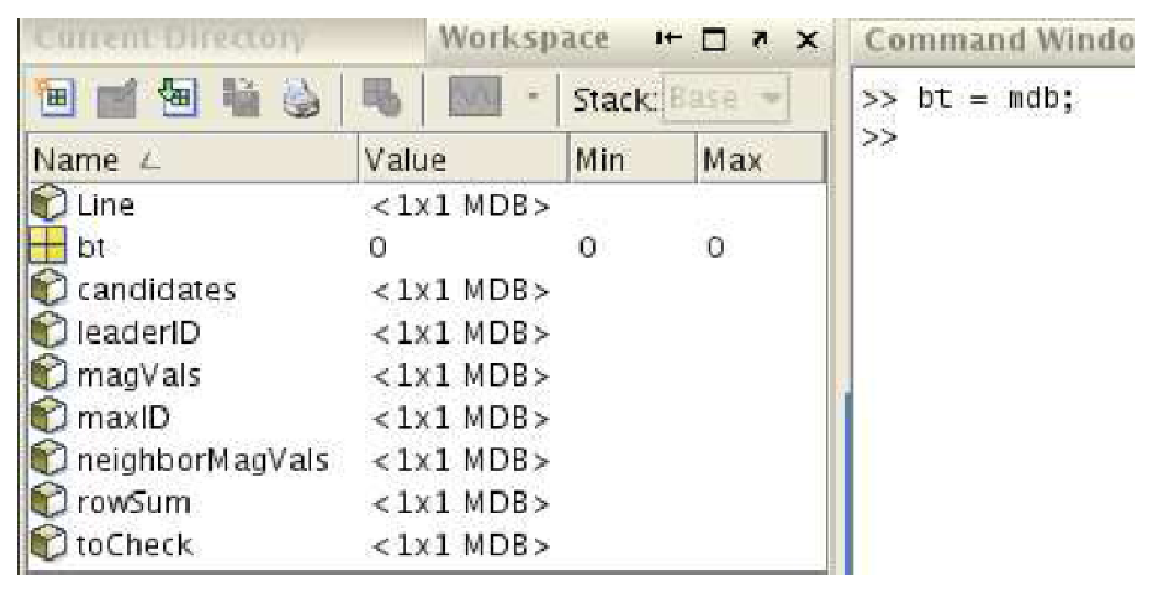
\includegraphics[scale=0.6]{fig/mdbInit}
}
\caption[MDB User Interface]{Starting the MDB debugger creates new objects in
the Matlab workspace for every macrovector in the program being debugged.}
\label{fig:matlab}
\end{figure}  

While the prototype implementation of MDB targets the MacroLab programming
environment, the principles behind the debugging approach can be applied to many
different macroprogramming abstractions. Because MacroLab uses a Matlab-like
syntax, the current implementation of MDB is designed to be used through the
Matlab command prompt. To debug the execution of a MacroLab program using MDB,
the user executed the {\tt mdb} command which starts up Matlab with the
workspace initialized with the macrovectors in the program being debugged as
shown in Figure~\ref{fig:matlab}. Table~\ref{table:commands} provides a summary
of the main commands offered by MDB\@.

\begin{table}[!htb]
  {
  \begin{tabular}{|l|l|} \hline
    Command & Description\\ \hline\hline
    tjump (\emph{t}) & change the state of the system to time \emph{t} \us \\
    tstep [(\emph{t})] & change the state of the system to next logged time [or current time + \emph{t}] \\ \hline
    lbreak (\emph{l}) & place a breakpoint at line \emph{l} \\
    lstep [(\emph{l})] & increment to the next line [or step \emph{l} lines] \\ 
    lcont & move forward to the next breakpoint \\ 
    lstatus & list all breakpoints \\
    lclear [(\emph{l})] & remove breakpoint [at line \emph{l}] \\ \hline
    isCoherent (\emph{x}, \emph{y}) & check if \emph{x} is coherent with \emph{y} \\
    diff (\emph{x}, \emph{y}) & compare views \emph{x} and \emph{y} of a vector
    \\ \hline
    alt (\emph{hc}, \emph{tl}) & produce a timeline by altering \emph{tl} using hypothetical change \emph{hc}\\
    getTime & get current debugger time \\ \hline
  \end{tabular}}
  \caption[Basic commands provided by MDB]{Basic commands provided by MDB. These commands allow the user to (1) navigate the trace temporally, (2) navigate the trace logically, (3) compare macrovectors, and (4) make hypothetical changes to the code.  
  }
  \label{table:commands}
\end{table}

\subsection{Logically Synchronous Views} \label{logical}

\emph{Logically synchronous views} allow the user to inspect and analyze the
distributed state of the system when all nodes are executing the same logical
operation, (i.e., the same line of code.)  MDB provides three commands for
generating and navigating through logical views: {\tt lbreak}, {\tt lcont}, and
{\tt lstep}.  These commands are used to debug logical errors such as Bug 1 from
Section~\ref{Bugs}, where the system fails to detect moving objects because of a
typo on line 8.  The user wants to first inspect the sensor values stored in
{\tt magVals} and so places a breakpoint on line 8 using the {\tt lbreak}
command: \\ {\small\tt\indent >> lbreak(8)}\\ {\small\tt\indent Breakpoint set
at
line 8}\\
The user then executes the {\tt lcont} command, which advances the state of the
application on all nodes until just before they execute the operation on line 8
for the first time:
\\ {\small\tt\indent >> lcont}\\
{\small\indent\tt At Line 8}\\
The programmer views the value of the {\tt neighborMag} macrovector by simply
typing
the variable name:\\
{\small\tt\indent >> neighborMag}\\
{\small\tt\indent neighborMag =}\\
{\small\tt\indent\indent(1,1)~~~~540}\\
{\small\tt\indent\indent(1,4)~~~~505}\\
{\small\tt\indent\indent(1,7)~~~~523}\\
{\small\tt\indent\indent\ldots}\\
Since node 1 has at least three neighbors with sensor readings above {\tt
THRESH}, the programmer expects it to be in an {\em active} neighborhood.
The programmer progresses past line 8 with the {\tt lstep} command: \\
{\small\tt\indent >> lstep}\\
{\small\indent\tt At Line 9}\\
and views the value of the {\tt active} variable:\\
{\tt\small\indent >> active}\\
This action reveals that {\tt active} is an empty vector, even though node 1 has
at least three active neighbors.  At this point, the programmer inspects line 8
of the macroprogram and finds that the logic of the program was specified
incorrectly: line 8 compares {\tt THRESH} to the {\tt magVals} variable instead
of the {\tt neighborMag} variable.

The key challenge to providing a logically synchronous view of macroprogram
execution is that the nodes may take different paths through the macroprogram,
but the system must still allow the user to step sequentially through the
macroprogram. MDB allows this by using an intuitive forward ordering of program
statements: when the user executes the {\tt lstep} command, MDB only advances
those nodes for which the next instruction has the lowest line number of all
nodes' next instructions.  More formally, $\mathbf{l}$ is defined to be the
vector of line numbers $l_i$ for each node $i$ in the current logically
synchronous view, and define $\mathbf{n}$ to be the vector of the next line
numbers $n_i$ that each node $i$ executed and logged immediately after line
$l_i$.  When the user executes the {\tt lstep} command, the next logically
synchronous view will be the vector $\mathbf{l'}$ of line numbers $l'_i$, which
are defined as

$$ l'_i =
\begin{cases}
  n_i & \mathrm{if~} n_i = min(\mathbf{n})\\
  l_i & \mathrm{otherwise}
\end{cases}
$$

\begin{figure}[t]
\centering{
  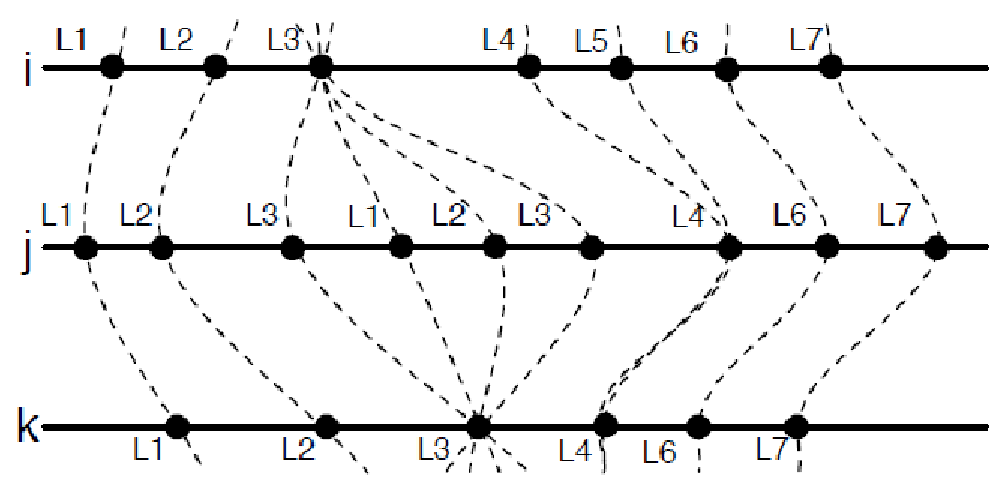
\includegraphics[scale=0.5]{fig/allBreakpoints}
\begin{macrolab}
   while( magVals < 10 )
     magVals = magSensors.sense()
   end
   if magVals > 3000
     magSensors.calibrate()
   end
   Display(magVals)
\end{macrolab}
}
\caption[Logically synchronous views]{Logically synchronous views (shown by dashed lines) depict nodes $i$,
  $j$, and $k$ progressing through the code in unison, even though node $j$
  executes the loop twice and only node $i$ executes line 5.}
\label{fig:allBreakpoints}
\end{figure}

Figure~\ref{fig:allBreakpoints} illustrates the effect of intuitive
linearization, where the solid lines show the sequence of statements that each
node executes in the example program, and the dashed lines illustrate the ten
logically synchronous views that MDB would create as a user executes the {\tt
  lstep} command.  In the first three views, all nodes progress through lines 1,
2, and 3 simultaneously. Node $j$ iterates through the loop twice, executing
lines 1, 2, and 3 again.  In the logically synchronous views, nodes $i$ and $k$
remain at line 3 until node $j$ exits the loop, at which point all nodes
progress to line 4 together, as illustrated by the dashed lines.  Similarly,
nodes $j$ and $k$ remain at line 4 in the logically synchronous views until node
$i$ finishes executing line 5, when the views show all three nodes progressing
to line 6 together. Thus, logically synchronous views depict all nodes
progressing through the code in unison, even though they may take different
paths through the code or execute the same lines of code at different times.

Logically synchronous views provide a convenient abstraction for navigating back
and forth through the logic of a macroprogram, but they are limited in that the
views of distributed state may include values that correspond to different
points in time. This could lead to {\em causally inconsistent} states being
presented to the user. For example, by the time node $i$ reaches line $L$, node
$j$ may already have passed line $L$ and sent $i$ a cache update. Thus, a
logically synchronous view at line $L$ would show nodes $i$ and $j$ in a
causally inconsistent state. Although all elements of the global state shown in
such a view are not causally consistent, the view itself is still useful for
debugging. In WENs, the user may also want to see distributed state at the
specific time that a physical event took place in the network.  For this reason,
MDB also provides temporally synchronous views, described in the next section.

The technique described above for representing branches and loops in logically
synchronous assumes that all nodes execute the same code and that no node fails
or blocks indefinitely on a variable. The first assumption is inherent in the
technique for stepping through non-sequential code sequentially and, therefore
limits the usability of the logically synchronous views in MDB while the second
assumption can easily be eliminated by monitoring for a node failure or
indefinite block when generating the next logically synchronous view in response
to an {\tt lstep}. In the event that no node's state can be updated based on the
technique above, yet all the nodes are not at the same macrocode line number,
any node that is not at the common macrocode line can be assumed to have failed
and be ignored in generating future logically synchronous views.

\subsection{Temporally Synchronous Views} \label{temporal}

\emph{Temporally synchronous views} allow the user to inspect and analyze the
distributed state of the system at a specific time.  MDB provides two commands
for moving forward and backward in time: {\tt tjump} jumps to a specific time,
and {\tt tstep} moves forward or backward by a given duration. These commands
can be used to debug configuration errors such as Bug 2, described in
Section~\ref{Bugs}, in which the mobile objects move by the nodes much more
quickly than the rate at which they sample from the sensors.  In this
experiment, the programmer observes an object moving through the network
approximately 0.4 seconds after execution started, but the object is not
detected by the network.  The
programmer jumps to this time using the {\tt tjump} command:\\
{\small\indent\tt >> tjump(400000)}\\
{\small\indent\tt At 400000 microseconds}\\
The programmer then
inspects the {\tt neighborMag} macrovector:\\
{\small\indent\tt >> neighborMag}\\
{\tt\small\indent neighborMag =}\\
{\small\tt\indent\indent(1,1)~~~~508}\\
{\small\tt\indent\indent(1,4)~~~~125}\\
{\small\tt\indent\indent(1,7)~~~~207}\\
{\small\tt\indent\indent\ldots}\\
The user can see that only one node has a sensor value above {\tt THRESH} at
that time time. Then the user steps forward in time by entering the {\tt tstep}
command:\\
{\small\indent\tt >> tstep}\\
{\small\indent\tt At 404129 microseconds}\\
When issued with no parameter, {\tt tstep} continually steps forward to the next
log entry.  The programmer notices that node 1's neighboring nodes do not read
from their sensors until long after the mobile object has left the vicinity,
indicating that the sampling frequency is not high enough.  This example
illustrates how temporally synchronous views allow the user to view distributed
state at the actual time a bug manifestation was observed.  This is particularly
useful in WENs, where bug manifestations may correspond to physical events that
do not correspond to the logic of the macrocode.
 
Temporally synchronous views allow the user to navigate through the execution
trace of a WEN, but are limited by the fact that the user must be able to
specify the exact times of interest.  Identifying the time that an interesting
event occurred to within milliseconds or microseconds can be a challenge,
especially when the timestamps do not necessarily correspond to the values of
any given wall clock.  For this reason, MDB also provides capabilities for {\em
historical search}, as described in the next section.

\subsection{Historical Search} \label{history}

\emph{Historical search} allows the user to inspect and analyze the historical
sequence of distributed system states without manually stepping forward and
backward through the code.  Like most source-level debuggers, the temporally
synchronous and logically synchronous views only show the user one state of the
system at a time. This requires the user to step forward and backward through
execution while trying to remember and correlate values from different states to
find the cause of a fault.  Historical search allows the user to operate over
the state of the system at all times at once, eliminating the need to step
forward and backward in time.

MDB allows the user to access the history of a macrovector by adding a new
dimension to it which represents time. For example, in the object tracking
application in Figure~\ref{code:PEG}, {\tt magVals} is a single-dimension
macrovector that is indexed by node ID\@. The value of {\tt magVals} at node $5$
and time $1000$ can be accessed with the command:\\ {\small\indent\tt >>
magVals(5, 1000)}\\ {\small\indent\tt ans =}\\ {\small\indent\indent\tt 17316}\\
Macrovectors conform to standard Matlab syntax even with the additional time
dimension, and standard Matlab operators can be applied to them.  This produces
a powerful programmatic debugging interface that can be used to search for the
manifestation of bugs.  Historical search can be used to find timestamps of all
instances of Bug 3 in which more than one leader was detected, using a single
command: \\ {\small\indent\tt >> find(numel(leaders(:, :)) > 1)}\\
{\small\indent\tt ans =}\\ {\small\indent\indent\tt 17317316}\\
{\small\indent\indent\tt
39824496}\\
where {\tt numel} is a standard Matlab operation that returns the number of
elements in a vector.  In this scenario, the developer finds that the IDs of
more than one node were stored in the {\tt leaders} macrovector at two times
during program execution.  To identify the cause of the bug, the programmer then
jumps to one of these times using the command:\\ {\small\indent\tt >>
tjump(17317316)}\\
{\small\indent\tt At 17317316 microseconds}\\
\begin{figure}[t]
\centering{
  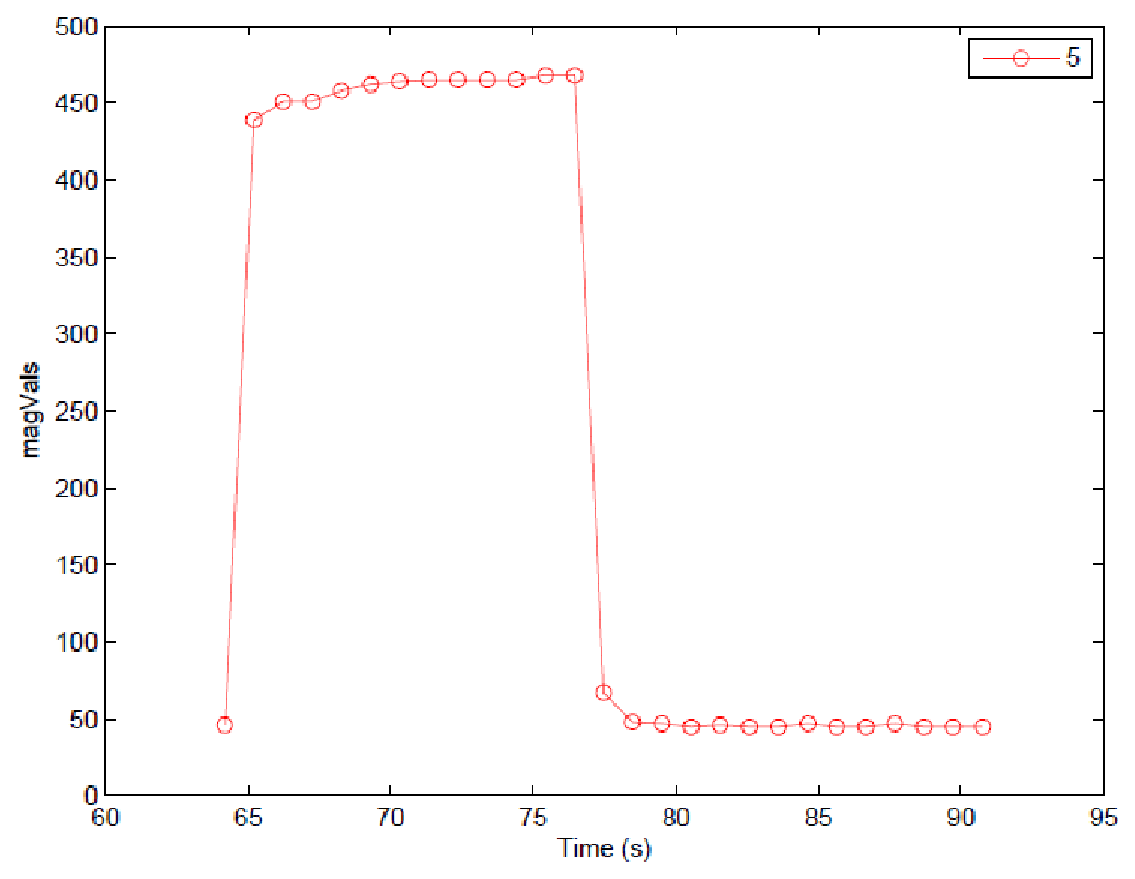
\includegraphics[width=0.5\columnwidth]{fig/plot}
}
\caption[Example plot]{MDB's views of distributed state can be combined with Matlab's rich
  plotting and analysis tools.  This figure is the result of a single debugging
  command: {\tt plot(magVals(5, :))}}
\label{fig:examplePlot}
\end{figure}
MDB's historical search functionality allows the user to exploit Matlab's rich
plotting and analysis tools.  For example, the command\\ {\small\indent\tt >>
plot(magVals(5,:))}\\ produces the graph shown in Figure~\ref{fig:examplePlot}
that contains all sensors values read by node 5.  Historical search provides a
convenient mechanism for searching through and analyzing the historical sequence
of distributed system state.

\subsection{Hypothetical Changes} \label{views}

MDB allows the user to observe how {\em hypothetical changes} to a macroprogram
would affect distributed state, without redeploying and executing the new
code. This functionality is useful for testing whether a particular change will
fix all occurrences of a bug that appeared in a given execution trace. As a
proof-of-concept, MDB currently provides four hypothetical changes that highlight the
effects of adding process and data synchronization primitives to a macroprogram:
(i) a hypothetical barrier (ii) hypothetical cache coherence (iii) a
hypothetical time delay, and (iv) hypothetical cache expiration.

The original execution trace that was collected during program
execution is called the {\em base timeline} and is denoted $bt$.
Hypothetical changes are applied to the base timeline to generate
an {\em alternative timeline} denoted $at$.  For example, the programmer
could make a hypothetical change to a program by setting {\tt magVals
  = 0} at line
7 by executing the {\tt alt} command:\\ {\small\indent\tt >> at =
  alt('magVals = 0', 7, bt)}\\ This command would produce {\tt at} by
modifying {\tt bt} such that {\tt magVals} is always set to $0$ at line 7.
The value of a macrovector in this alternative timeline can be viewed by
passing a handle to the timeline as an optional last parameter when
indexing that macrovector.  For
example, a user can view node 7's value of {\tt
  magVals}
at time $10000$ in the alternative timeline by executing the commands:\\
{\tt\small\indent >> magVals(7, 10000, at)}

\subsubsection{Hypothetical Barrier} \label{barrier}

A \emph{barrier} is a point in the source code that all nodes must reach before
any node can proceed.  The \emph{hypothetical barrier} illustrates how the
distributed state of the system would change if a barrier were placed at a
particular line of macrocode.  For example, the user can use hypothetical
barriers to test whether a barrier at line 12 in the example program
from Figure~\ref{code:PEG} would fix Bug 3 from Section~\ref{Bugs}.  To do so, the
programmer first creates an alternative timeline with a hypothetical barrier at
line 12 using the command:\\ {\small\indent\tt >> hb = alt('barrier()', 12,
  bt)}\\ The user then checks if multiple leaders still arise with a
barrier by apply the same command that was used in Section~\ref{history} to the
new timeline:\\ {\tt\small\indent >> find(numel(leaders(:, :, hb)) >
  1)}\\ Because this command no longer returns any timestamps, the user
concludes that applying a barrier to line 12 would fix Bug 3.  Thus, this
hypothetical change allows the programmer to test whether this code
modification, with respect to the given trace, fixes all occurrences of this
bug, some occurrences, or no occurrences, without the need to redeploy, execute,
and test the code.

The semantics of a hypothetical barrier is illustrated using the example
execution timelines shown in Figure~\ref{fig:barrier}.  MDB first creates a
logically synchronous view at line 12, as illustrated by the dashed line.  If
the nodes had implemented a barrier, the state of the system would be identical
to the state represented by this logically synchronous view, except that
additional cache update messages would have been received.  Specifically, any
node $a$ that waited at the barrier would have received all messages from
another node $b$ that were sent before $b$ reached line 12 and that were
received before all nodes reached line 12. Thus, MDB creates the hypothetical
barrier by updating the state of the logically synchronous view at line 12 with
all such cache update messages.  This hypothetical change to the order in which
cache update messages are received is illustrated by a dashed arrow in
Figure~\ref{fig:barrier} to illustrate the difference between the messages that
were received in the real execution trace $bt$, and the messages that were
received in the alternate timeline $at$. The distributed state resulting from
this message re-ordering is the view of a hypothetical barrier applied to line
12.

\begin{figure}[t]
\centering{
\subfigure[Hypothetical Barrier]{
  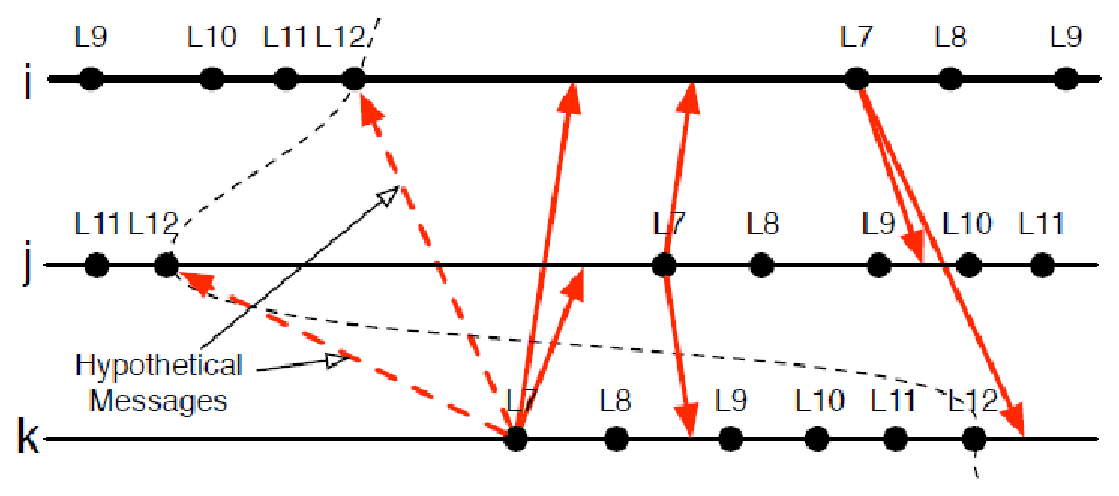
\includegraphics[scale=0.5]{fig/barrier}
  \label{fig:barrier}
}
\subfigure[Hypothetical Time Delay]{
  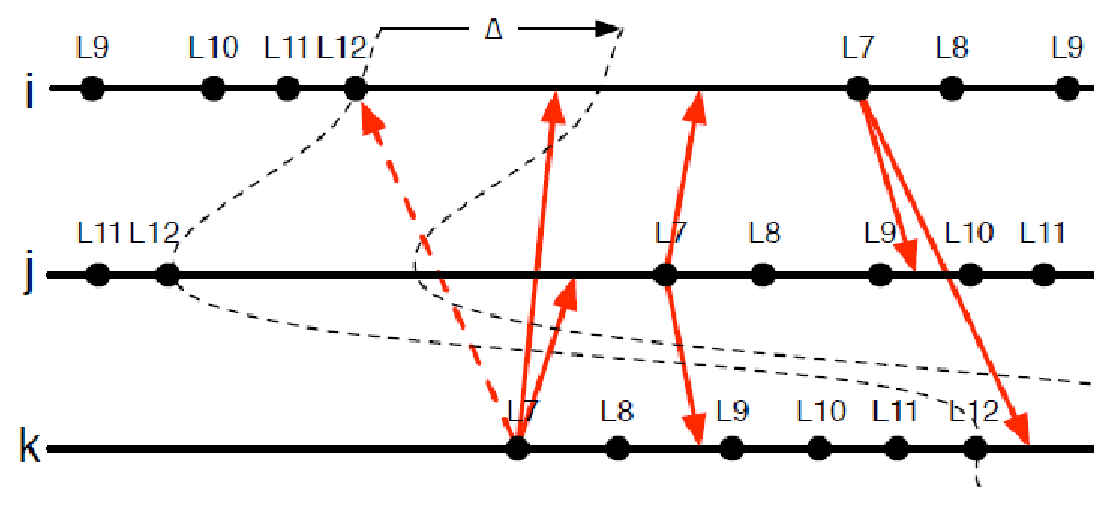
\includegraphics[scale=0.5]{fig/wait}
  \label{fig:deltat}
}
\subfigure[Hypothetical Cache Coherence]{
  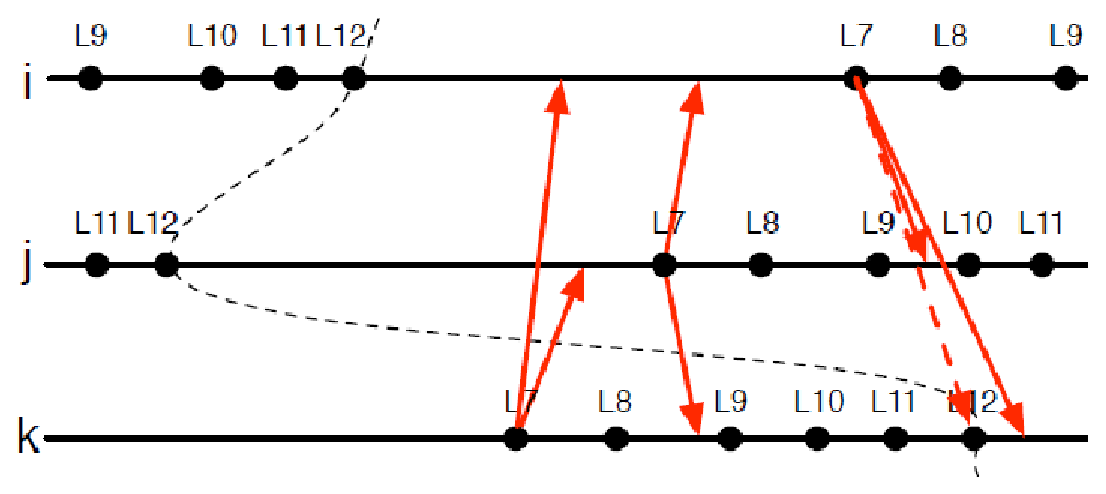
\includegraphics[scale=0.5]{fig/cacheCoherent}
  \label{fig:coherent}
}
\caption[Hypothetical Changes]{MDB emulates the effect of hypothetical code changes by
    reordering messages appropriately.  Solid arrows illustrate message
    reception in an actual execution trace.  Dashed arrows illustrate how these
    messages are re-ordered to emulate the effect of hypothetical changes to the code.}
\label{fig:hypothetical}
}
\end{figure}

\subsubsection{Hypothetical Time Delay} \label{delay}

Barriers are expensive operations and are not always desirable in WENs due to
their high message cost.  A cheap alternative is to have all nodes wait for any
cache updates to arrive for only a fixed period of time before continuing
execution.  If execution on all nodes is already synchronized or is otherwise
known to be unsynchronized by a bounded duration, this approach may provide
sufficient data synchronization guarantees.  The \emph{hypothetical time delay}
produces the distributed state that would have been produced if a time delay of
$\Delta t$ were inserted at a particular point in the macrocode. The programmer
could create a hypothetical time delay using the {\tt deltat} command:\\
{\small\indent\tt >> dt = alt('deltat(10)',12, bt)}\\ {\tt deltat} takes a
parameter to indicates the delay $\Delta$t in milliseconds.  To create the
hypothetical time delay, MDB first creates a logically synchronous view on line
$12$. Then, the distributed state is updated with any cache update messages
received by a node withing the $\Delta$t of the time it reached line 12.
Figure~\ref{fig:deltat} illustrates that a hypothetical time delay applied at
line 12 would cause the message sent from line 7 of node $k$ to update the state
of node $i$ after executing line 12.

\subsubsection{Hypothetical Cache Coherence} \label{coherent}

\emph{ Hypothetical cache coherence} shows the hypothetical distributed state if all
caches were coherent at a given time. This view can be produced with the
command:\\ { {\small\indent\tt >> cv = alt('coherent()', 12
    bt)}}\\ To create hypothetical cache coherence, MDB rearranges any cache updates
that were sent before, but received after the line of code
specified. Figure~\ref{fig:coherent} illustrates how message reception is
altered by the command above: the message from node $i$ is received at node $k$
on line 12, because it was sent before $k$ finished executing line 12.  Perfect
cache coherence is expensive to implement because it requires two-phase locks to
be acquired on all cached versions of a variable before any new values can be
written to it.  If hypothetical cache coherence makes a bug manifestation disappear,
the user may attempt to use end-to-end reliability for cache updates,
low-latency communication protocols, or other mechanisms that will improve, but
not guarantee, cache coherence.

\subsubsection{Hypothetical Cache Expiration} \label{expiration}

\emph{Cache expiration} is the process of invalidating a cached copy of a value once it
becomes too old.  This is cheaper to implement than perfect cache
coherence, but it also provides few correctness
guarantees because the original value may change before the cached copies of the
old value expire.  Furthermore, when nodes run asynchronously and aperiodically
in a network, it can be difficult to decide when to expire cache entries.
Expiring too quickly can result in insufficient data, but expiring too slowly
can result in the use of stale values.  \emph{Hypothetical cache expiration} shows
the hypothetical state that would result if cache expiration were used at a
given line of code, with a particular expiration time.  This view helps
the user evaluate the effect of different expiration times and can be created
using a command such as:
\\
{\small\indent\tt >> ev = alt('expire(100000)', 12, bt)}\\
The values in the view are produced by finding the last value written
to each element of the macrovector in the time interval $[t-t_{e},~ t]$
where $t$ is the time the node executed line 12 in the current
instance of the logically
synchronous view and $t_{e}$ is the expiration time, in
this case 100000\us.  If an element has had no value written to it
within that time interval, the resulting view has a $NaN$ value for
that element. 

\section{The MDB Implementation} \label{implementation}

This section describes the implementation of MDB, including the collection
of execution traces (Section~\ref{traces}), how MDB Lite reduces energy cost
(Section~\ref{mdbLight}), how timekeeping is performed on data traces
(Section~\ref{time}) , how MDB's global views and historical searches are
implemented using these data traces (Section~\ref{genViews}), and how
hypothetical changes are emulated by creating modified copies of these data
traces (Section~\ref{genAlt}).
 
\subsection{Creating Execution Traces} \label{traces}

MDB is a post-mortem debugger, which means that it must collect execution traces
at run-time that will be analyzed after execution is complete.  Most post-mortem
debuggers create \emph{event traces}: they log all non-deterministic events such
as interrupts, I/O, and messages.  These event traces are sufficient to recreate
the state of the system at any point of the original execution using
\emph{execution replay}.  In contrast, MDB creates \emph{data traces}: it logs
all changes to the system state, including writes to variables and changes to
the program counter.  Event traces generally produce shorter logs than data
traces because events are relatively rare while state changes occur with every
line of code executed, especially for traditional distributed applications that
are compute intensive but have relatively little I/O or network communication.
In contrast, each line of a macroprogram may correspond to many machine
instructions, I/O operations, and network events.  Therefore, data traces are
more efficient than event traces for logging macroprogram execution.

MDB log entries consist of the (macro)program counter, the variable location and
value being written, a $48 \ bit$ microsecond-accurate timestamp, and the
sequence number.  The sequence number helps correlate variable write events
with remote cache events of that same value, since message transmission and
reception are not logged.  After execution is complete, the logs are retrieved
from the nodes using the collection tree protocol from the TinyOS source tree,
although any data collection protocol can be used.

To minimize interference with the application, MacroLab logs data in two phases:
first in RAM and then to external flash. While the MacroLab application is
executing, trace entries are stored in a circular RAM buffer, requiring only 105
machine instructions per log.  Then, when the node has no more instructions to
process, and right before it enters sleep mode, the RAM buffer is dumped to
external flash, which takes approximately 50\ms.  This approach reduces MDB's
interference with the application by reducing contention for the CPU\@.  One
disadvantage of this approach, however, is that any log entries in the RAM
buffer may be lost if the node crashes.  All logging code required for MDB is
automatically added by the MacroLab compiler when the debugging option is
enabled.

The external flash is 1\mb in size, and when it is full the earliest trace
entries are overwritten.  One advantage of MDB's use of data traces is that old
trace entries can be overwritten when the external flash is full.  In contrast,
entries in an event trace cannot be overwritten because all events from the
beginning of execution are required for execution replay.  Therefore, systems
that collect event traces must use checkpointing techniques, which can introduce
additional overhead~\cite{Wittie1986}.

\subsection{MDB Lite} \label{mdbLight}

MDB Lite is a light-weight version of MDB that conserves energy by not writing
log entries to the external flash, although all other logging code is included
in the microprograms and is identical to MDB\@.  Furthermore, MDB Lite emulates
the process of writing to flash by using a hardware timer to turn off the
appropriate interrupts for the appropriate period of time.  The logging commands
and flash emulation ensure that the timing and memory characteristics of a
program are the same when executing MDB and MDB Lite.  Thus, MDB Lite cannot be
used for debugging, but it can be enabled during the deployment phase to reduce
energy overhead while also eliminating the possibility of heisenbugs: a change
in the manifestation of bugs when the debugger is enabled or disabled.  The user
can toggle between MDB and MDB Lite to enable or disable debugging.

\subsection{Distributed Timekeeping} \label{time}

After a program executes and the logs are collected, MDB must ensure that the
timestamps in the logs are \emph{causally consistent}: any event $e$ that causes
event $e'$ must have a smaller timestamp than $e'$.  Distributed time keeping is
a challenging problem because nodes do not share a common clock, and is the main
distinguishing feature between debugging on a distributed system and debugging
concurrent threads on a single machine or a shared memory multiprocessor (SMMP).
MDB adopts a well-known approach that is sometimes called the \emph{Lamport}
algorithm: all logs are timestamped with a value from the node's microsecond
counter, and clock skew is accounted for by enforcing that a receiver's local
time when a message is received is greater than the sender's local time when the
message was transmitted.  Since message passing is typically the only form of
interaction between nodes, this approach guarantees that any events on the
sender have an earlier timestamp than events they might cause on the receiver.
Any distributed timekeeping scheme that satisfies this property is said to
support \emph{Lamport time}~\cite{Lamport1978}.  Other timekeeping schemes such
as vector clocks have more precise causal
semantics~\cite{Mattern1989,Fidge1991}.  MDB's use of the Lamport algorithm
occurs off-line after the logs are collected, which eliminates the need for any
run-time overhead due to on-line time
synchronization~\cite{Elson2002,Maroti2004}.  One disadvantage of this approach
is that all nodes must receive periodic messages from neighboring nodes.  In a
partitioned network where some nodes do not have radio connectivity with other
nodes, the logs cannot be made causally consistent.  This is the case for all
distributed systems, and not a limitation specific to MDB.

Distributed timekeeping in WENs is complicated by the fact that nodes can also
interact through their sensors and actuators: two nodes can sense the same
stimulus, or a node's sensor reading can be affected by another node's actuator.
This causal relationship is not explicit in the program, cannot be verified at
run time, and cannot be enforced by the Lamport timekeeping algorithm. Such node
interactions through events external to the synchronization messages is called
\emph{anomalous behavior} by Lamport, who suggested physical clocks to eliminate
this limitation.  Empirical studies of the CPU clocks are performed on the
\tmotesky nodes and found an average clock skew of 139\us/$s$, similar to the
observations mentioned in RBS~\cite{Elson2002}. The inherent uncertainty of
sensor readings on the same nodes is measured to be about 20\ms, which is the
average time required for the ADC to digitize the analog readings from the
sensors, plus software overhead.  Thus, a minimum message rate of about one
message every 2 minutes is required to prevent clock skew from growing larger
than the inherent uncertainty on sensor reading timestamps.  The minimum message
rate may even be much larger when measuring physical stimuli such as temperature
or object mobility that change with periods much lower than 20\ms.

\subsection{Generating Global Views} \label{genViews}

Once the execution traces are retrieved and synchronized, MDB can use them to
create views of any system variable at any given time.  To view the value of
variable $x$ at time $t$, MDB indexes the trace of the node on which variable
$x$ was logged and retrieves the last value written before time $t$.  For
example, to produce the value of node $k$'s element of the {\tt magVals} vector
at time $1000$, the system may retrieve the value that was written to {\tt
magVals} by node $k$ at time $998$.  This basic functionality helps implement
MDB's logically synchronous views, temporally synchronous views, and historical
search.

Logically synchronous views are implemented using an {\tt lline} vector which
stores all the line numbers at which a breakpoint has been placed and an {\tt
ltime} vector which stores a time for each node to indicate MDB's location in
its trace. When the user enters {\tt lbreak} with a line number, the line number
is appended to {\tt lline}. When the user enters {\tt lstep}, MDB identifies
which nodes executed the next line of the macroprogram next and sets the value
of {\tt ltime} for those nodes to be the time when the node finished executing
that line. When the user executes {\tt lcont}, MDB executes {\tt lstep}
repeatedly until the macrocode line matches one of the values in {\tt lline}.

Temporally synchronous views are implemented using a variable called {\tt ttime}
which stores the parameter passed to {\tt tjump}. {\tt ttime} is updated when
the user issues the {\tt tstep} command. If the user views a macrovector after
{\tt ttime} has been set, the view of the macrovector is generated by searching
through the trace of each node for the last state update to the macrovector at
or before {\tt ttime}. Historical search is implemented by searching through the
execution traces for all writes to the macrovector specified by the historical
search.

MDB uses a special $NaN$ value to represent any value in a logically synchronous
or temporally synchronous view that does not exist in the logs.  This situation
occurs in a temporally synchronous view, for example, when a node fails or stops
executing and the log from that node does not contain values beyond a certain
point in time.  It may also occur in logically synchronous views, for example,
if a node blocks on a variable indefinitely or dies and its log has fewer
instances of a particular line number than the logs of other nodes.

\subsection{Generating Hypothetical Changes} \label{genAlt}

\begin{figure}[t]
  \centering{
    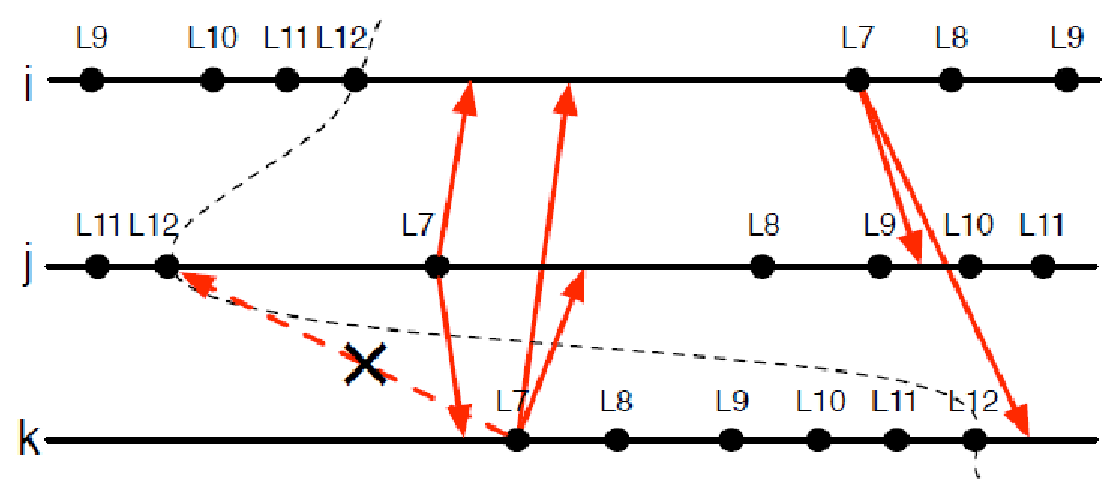
\includegraphics[scale=0.5]{fig/grandfather}
  }
  \caption[Grandfather paradox]{A hypothetical barrier cannot be applied in this
  scenario because the hypothetical advancement of the message from node $k$ to
  node $j$ would create a dependence cycle.}
  \label{fig:grandfather}
\end{figure}

Hypothetical changes are made by modifying an initial timeline denoted
{\tt it} to generate an alternate timeline denoted {\tt at}. This
process involves two phases: (1) applying hypothetical changes to {\tt
  it}, and (2) propagating the hypothetical changes into the
future. MDB carries out the first stage of alternative timeline
generation by copying all the values from {\tt it} into a new timeline
{\tt at}. Then, it generates logically synchronous views at each
instance of line $l$ specified by the user and MDB modifies the cache
update times based on the hypothetical change specified, as described
in Section~\ref{views}.  For example, to implement the hypothetical
barrier depicted in Figure~\ref{fig:barrier}, MDB would reorder the
trace entries in the new timeline {\tt at}, such that the message from
line 7 of node $k$ is received by nodes $i$ and $j$ when they reach
the barrier.  After the message reordering is complete, MDB propagates
this change into the future by re-executing the instructions
corresponding to every subsequent log entry in $at$, in the order of
their timestamps.  Thus, MDB re-executes the instructions logged in
the original execution trace to propagate the state from the
hypothetical change into all future states.  After re-executing each
line of code, MDB re-creates a new trace entry and adds it to the
alternative timeline {\tt at}.  Thus, alternative timeline {\tt at}
should have exactly the same timestamps on all log entries as the
original timeline {\tt it}, but might have slightly different values.

When a node reads from a sensor, MDB retrieves the sensor reading that
was collected in the original execution trace.  MDB does not attempt
to generate simulated sensor values based on a model of the stimulus.
Therefore, creation of the alternative timeline cannot proceed once
the control flow of execution diverges from the control flow observed
in the original execution trace.  Thus, hypothetical changes can only
be propagated into the future insofar as they do not change control
flow; any request for a view of the alternative timeline after control
flow changes produces the $NaN$ value, to indicate that the
view cannot be generated.  This limitation could be overcome by
incorporating simulation and sensor models into MDB, but this is
beyond the scope of this dissertation.

In addition to control flow changes, alternative timeline generation also fails
in certain instances when the user specifies a hypothetical change that results
in a \emph{causality cycle}: an event $e$ that is caused by event $e'$ reordered
to occur before $e'$.  For example, in Figure~\ref{fig:grandfather}, the
hypothetical barrier applied to line 12 would cause message $m$ from line 7 of
node $k$ to be received before message $m'$ is sent at line 7 on node $j$.
However, this produces a causality cycle because message $m'$ is also received
by node $k$ before it sends message $m$.  This scenario is called the
\emph{grandfather paradox}.  MDB checks for the grandfather paradox during the
creation of alternative timelines, and all subsequent values that are causally
related to $m$ or $m'$ are assigned the $NaN$ value.


\section{Macroprogramming Properties for MDB} \label{language}

While MDB is currently implemented for MacroLab, its principles apply to other
macroprogramming systems. This section defines the language and system
properties necessary to support various aspects of MDB and identify other
macroprogramming systems that share these properties.

\par{\bf High-level abstraction. } The high-level programming abstraction of
  MacroLab concisely describes complex system states in a small number
  of lines of code and variables. This allows for efficient logging on
  resource-constrained devices. All macroprogramming abstractions, by
  definition, allow for such a succinct
  descriptions~\cite{Mainland2008,Newton2004,Welsh2004,Kothari,Greenstein2004}.  

\par {\bf No message passing. } MacroLab forbids user-written
  message passing, instead managing all communication in the
  run-time system. MDB can thus log only cache update messages.  
  Systems such as Hood~\cite{Whitehousea}, Pleiades~\cite{Kothari},
  COSMOS~\cite{Awan2007}, and Semantic Streams~\cite{Whitehouse} also abstract away
  message passing from the programming model.

\par {\bf Clear mapping from macro-code to micro-code. } This is
essential to log the ends of macrocode lines in microcode. Most
macroprogramming systems, such as~\cite{Kothari} translate the
macrocode statements into appropriate blocks of microcode and
therefore possess this property.

\par {\bf In-order message delivery. } This enables cache updates from a
  given node to be received in the order they occurred in locally. Most
  macroprogramming systems are built on this assumption~\cite{Birman1994}. If
  not, sequence numbers can be used to to prevent out-of-order cache
  updates. 

\par {\bf Sequential imperative language. } 
  MacroLab allows logically synchronous views to be generated where the
  user can place breakpoints and step through code. This property is
  supported by all sequential imperative macroprogramming systems, such as
  Marionette~\cite{Whitehouseb}. 

\par {\bf Data caching. } Data caching, in the form of neighbor reflections,
  yields Lamport time stamps without additional logging. This property
  also makes hypothetical views both possible and useful since they show
  how data caching would be affected by application changes. All
  macroprogramming abstractions that support data caching, such as
  Hood~\cite{Whitehousea}, provide this property. 

\par {\bf Single machine abstraction. } MDB displays the state of the
system as the state of the macrovectors if they were centralized. This
requires the system to provide a single machine abstraction to the network.
Systems such as RuleCaster~\cite{Bischoff} also possess this property.

\par {\bf Data-centric. } The data-centric nature of MacroLab enables data
traces, rather than event traces, to be logged. Semantic
Streams~\cite{Whitehouse}, COSMOS~\cite{Awan2007}, and TinyDB~\cite{Madden} are
similar data-centric languages. 


\section{Evaluation} \label{evaluation}

MDB is evaluated in two phases. First, it is shown that data traces are more
effecient for macrodebugging than the traditional approach of creating event
traces.  Then, the RAM, flash, energy, and CPU cycle overhead of MDB\@ is
evaluated.

\begin{figure}[!htb]
  \centering
  \includegraphics[scale=1.2]{fig/testbed}
  \caption[Evaluation testbed with 21 Tmote Sky motes]{MDB is evaluated on three
  macroprograms by running them on a 21 node testbed. Light sensors and a
  projector created the sensor stimuli.}
  \label{fig:testbed}
\end{figure}

\subsection{Experimental Setup}
The evaluations were carried out on a testbed with 21 TMote Sky nodes with
photoresistor sensors (Figure~\ref{fig:testbed}). Since all the nodes in the
testbed are within one hop of each other, their communication ranges are
artificially limited by modifying the packet reception module of the CC2420
radio. Nodes are restricted to communicate with neighbors next to them
vertically, horizontally, and on the two diagonals.  To collect additional data
that could not be obtained from the testbed, the node-level Cooja network
simulator~\cite{Osterlind2006}, which makes use of the
MSPSim~\cite{Eriksson2007} TMote Sky simulator, is used.  The microcode
executing on the nodes in the Cooja simulator is exactly the same microcode that
executes on the real \tmotesky hardware.

MDB is evaluated with three macroprograms.  The first application is PEG,
described earlier (Figure~\ref{code:PEG}), for which the movement of objects is
emulated using the light sensors by moving a white circle on a black background
that was projected from a laptop onto the testbed. The intensity of the circle
decreases radially outward to emulate the effect of varying sensor readings by
nodes that detect the object.  The second application is Surge
(Figure~\ref{code:Surge}), which is a simple data collection application that
periodically samples from a sensor and displays the readings at a base station.
The third is an acoustic monitoring application (Figure~\ref{code:acoustic}),
which first senses from a microphone sensor, and depending on the number of
neighbors that also heard a sufficiently loud sound, samples from a second
high-fidelity microphone, stores the values, and reports them to the base
station.  The sensor values for both of these applications are generated using
the photoresistors on the nodes.

% \begin{figure}[t]
% \begin{macrolab}
% every(uint16(1000))
%  lightVals = lightSensor.sense();
%  basedisplay(lightVals);
% end
% \end{macrolab}
% \caption[The macroprogram for Surge]{Surge reads sensor values and displays them
% at the base station.}
% \label{code:surge}
% \end{figure}

\begin{figure}[t]
\begin{macrolab}
every(uint16(1000))
 trigger = microphone.sense();
 meanTrigger = mean(neighborTrigger, 2);
 candidates = find(meanTrigger > THRESHOLD);
 soundLog(candidates) = microphoneHF(candidates).sense();
 baselog(soundLog);
end
\end{macrolab}
\caption[An acoustic monitoring application in MacroLab]{The acoustic monitoring
application reads values from a microphone and reads from a higher-fidelity
microphone on nodes whose neighborhoods detect high average noise levels.}
\label{code:acoustic}
\end{figure}

\subsection{Data vs. Event Logging} \label{dataEvent}

\begin{figure}[t]
  \centering
  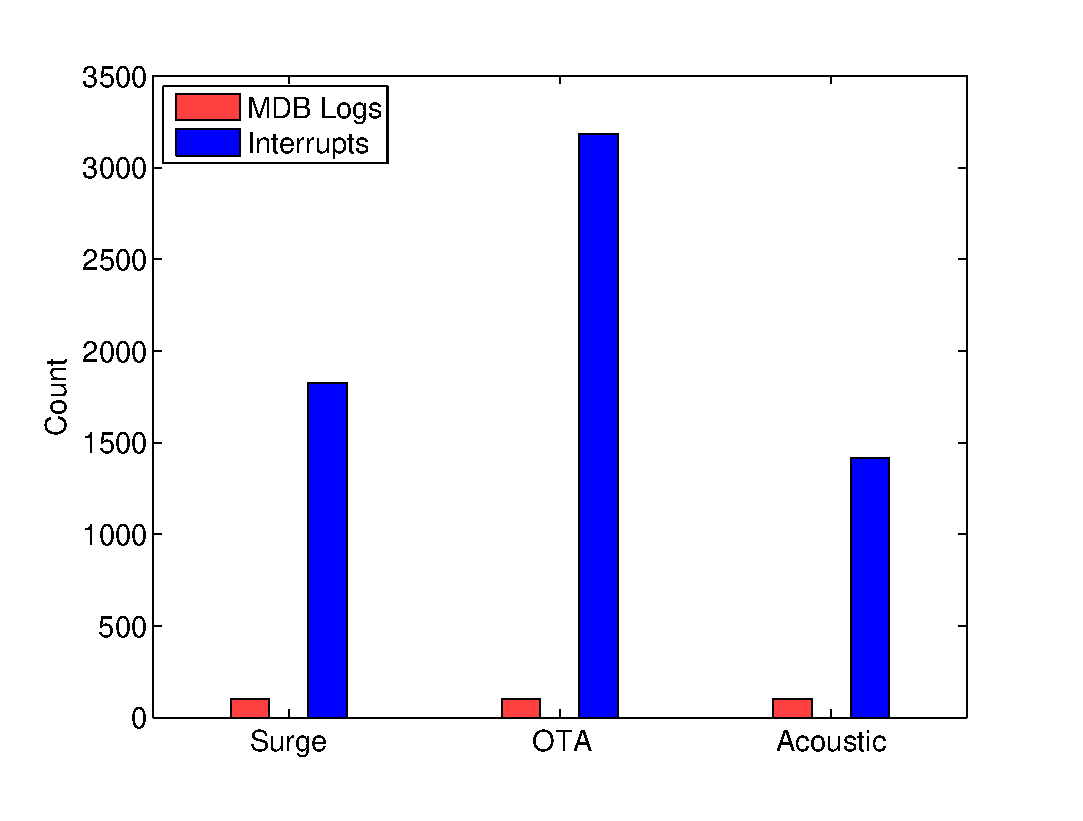
\includegraphics[width=0.6\columnwidth]{fig/interruptvsMLLogger}
  \caption[Number of interrupts generated per 100 data states written to
  flash]{Number of interrupts generated per 100 data states written to
  flash. WEN applications produce 14--32 times more interrupts and message
  events than macroprogram state updates.}
  \label{fig:interruptvsMLLogger}
\end{figure}

The cost of creating data traces is evaluated by counting the number of logging
statements required to record all variable writes and program counter changes
for a single run of each of the three macroprograms. This count is compared to
the number of interrupts that would need to be logged to create an event trace
of the same program execution.  Since the interrupts generated on real hardware
could not be counted without changing the timing characteristics of the program,
these values were obtained by analyzing the programs as they executed on the
Cooja network simulator.  Figure~\ref{fig:interruptvsMLLogger} shows that, for
these applications, the number of hardware interrupts is 14--32 times larger
than the number of updates to macroprogram state.  These results clearly show
that MDB's approach of collecting data traces is much more efficient for
macroprograms than the traditional approach of collecting event traces.

\subsection{RAM and Flash Overhead} \label{overhead}

\begin{figure}[!htb]
  \centering
  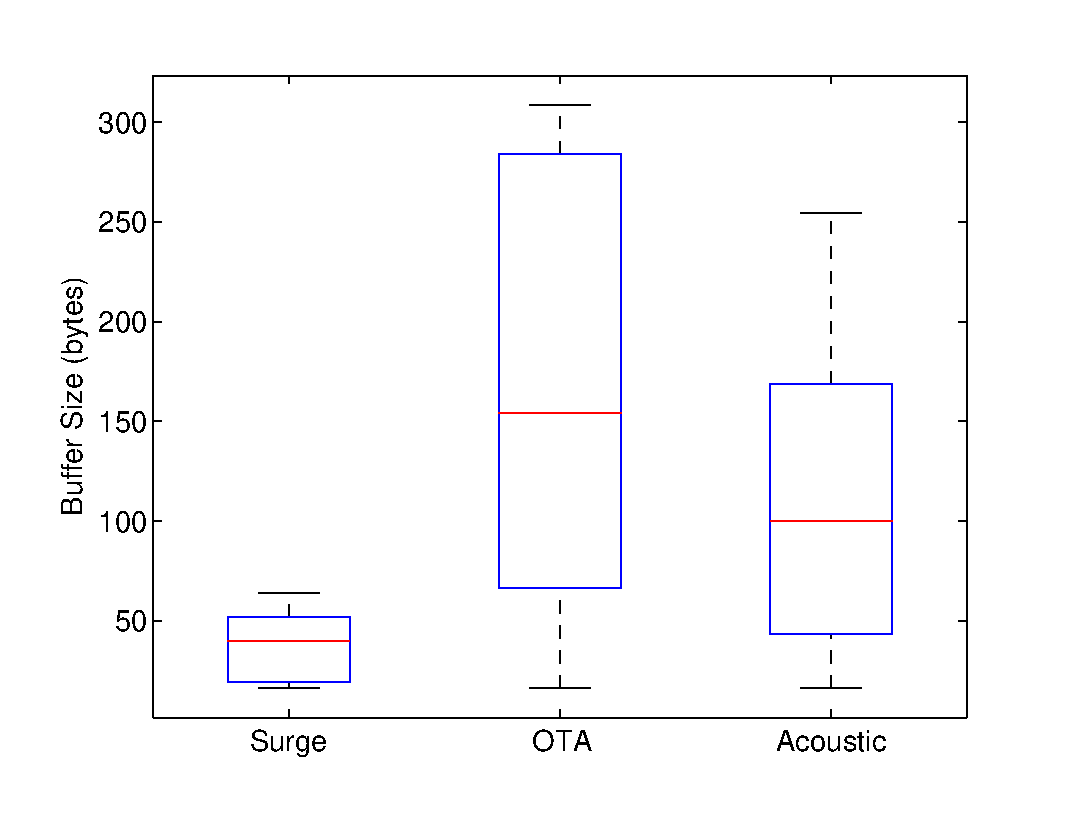
\includegraphics[width=0.6\columnwidth]{fig/bufferSize}
  \caption[RAM Overhead]{Log data is stored temporarily in RAM before being written to flash.
    In the experiments, no node needed more than 304 $Bytes$ of RAM\@. The box plot
    shows the minimum, lower quartile, mean, upper quartile, and maximum
    values.}
  \label{fig:bufferSize}
\end{figure}

\begin{table}
  \centering
  {
    \begin{tabular}{|l|r|r|} \hline
      Application & Flash ($Bps$) & Wraparound ($hr$)\\ \hline\hline
      Surge & 31 & 9 \\ \hline
      Accoustic & 187 & 2 \\ \hline
      PEG & 288 & 1 \\ \hline
  \end{tabular}}
  \caption[Flash memory consumption]{Flash memory consumption is low enough to debug hours of
      execution. The buffer is circular, so it can always store data to debug the
      last few hours of execution.}
  \label{table:flashCapacity}
\end{table}

Memory is not typically a concern for traditional debuggers that execute on PCs,
but WENs are composed of highly resource-constrained devices and efficient
memory usage is essential to making MDB practical in this domain. The amount of
memory MDB requires is measured by instrumenting the RAM buffer portion of the
logger and tracking the maximum difference between the head and tail pointers of
the circular buffer. Figure~\ref{fig:bufferSize} depicts box plots that show the
minimum, maximum, mean, and the lower and upper quartiles of RAM consumption for
each of the three test applications executing on a 21 node testbed. This data
reveals that MDB has modest RAM requirements, and needs to store a maximum of
304 $Bytes$ of data, while the \tmotesky nodes have about 10\KB of RAM
available.

The amount of Flash memory required by MDB to store the complete data traces for
each of the three applications was measured.  Table~\ref{table:flashCapacity}
shows that the applications store less than 300 $Bps$ to the flash.  At these
rates, simple applications such as Surge can collect logs for several hours
before exhausting the $1 \ MB$ of external flash available on the \tmotesky.
More complicated applications such as PEG and acoustic monitoring may exhaust
the flash after about one and a half hours. Thus, bugs in these applications
must be detected within one and a half hours in order to debug them before the
log entries are overwritten.

\subsection{CPU Overhead} \label{CPUoverhead}

The effect of MDB on the execution speed is evaluated by counting the logging
instructions executed during a particular run of the three applications. Since
it was difficult to collect this information from the actual nodes without
substantially modifying the timing characteristics of the application, this data
was collected by running the application on the Cooja simulator. Since Surge has
no interaction between nodes, it is simulated using 1 node.  Acoustic monitoring
used 5 nodes and PEG used 10 nodes.  Figure~\ref{fig:execBreakdown} shows the
number of MacroLab application instructions and MDB logging instructions that
execute, as a percentage of the total execution time. The values in
Figure~\ref{fig:execBreakdown} are averages over all the nodes simulated in
Cooja. As Figure~\ref{fig:execBreakdown} shows, the MacroLab application code
executes for between 2\% and 6\% of the total execution time and the logging
code executes for less than 0.5\% of the total execution time.

\begin{figure}[t]
  \centering \includegraphics[width=0.6\columnwidth]{fig/execBreakdown}
  \caption[CPU Overhead]{MacroLab context constitutes less than 6\% of all code running on
      the nodes. Logging code constitutes less than 0.5\%.}
  \label{fig:execBreakdown}
\end{figure}

It takes exactly 105 machine instructions to log data to the RAM buffer.
Execution is minimal because on the MSP430 an instruction takes approximately
125 nanoseconds.  This means the logging overhead is about 13 microseconds.
This is extremely small when compared to the normal duty cycle of applications
written in MacroLab.

\subsection{Energy Consumption} \label{PowerConsumption}

MDB's energy consumption is evaluated by executing the PEG application, with the
senor being sampled every $10$ seconds, on the 21 node testbed and measuring its
average current draw over a period of $100$ seconds. This experiment is executed
with MDB, MDB-lite, and without MDB\@.  The experiment is repeated both with and
without low-power listening
(LPL)~\cite{Polastrea}. Figure~\ref{fig:mdbPowerConsumption} shows that an
application consumes 30\% more energy with MDB, when LPL is enabled with a sleep
interval of $1$ second.  This energy overhead is due to the process of saving
logs to the external flash chip. With MDB Lite, this overhead is reduced to only
0.2\mW or 0.9\%.  This is because MDB Lite does not write to flash, and the
timer-based implementation of MDB Lite allows the node to sleep when possible.
The overhead of MDB and MDB Lite when LPL is disabled is only 0.5\mW because the
node does not go into sleep mode in any of these implementations.

\begin{figure}[t]
  \centering \includegraphics[width=0.6\columnwidth]{fig/energy}
  \caption[Energy Consumption]{Without low-power listening enabled, applications
  consume 30\% more energy with MDB enabled, but only 0.9\% more energy with MDB
  Lite. }
    \label{fig:mdbPowerConsumption}
\end{figure}

\subsection{Discussion} \label{discussion} 
%
The effectiveness of MDB as a CPS debugger depends on two factors: (i) the
usefulness of the debugging abstraction and (ii) the efficiency of trace
logging. The first factor is addressed by demonstrating that the features of MDB
can be used to debug three classes of bugs in macroprograms
(Chapter~\ref{Interface}). MDB, by its very nature, does not enable the
debugging of bugs in layers below the application layer. For example, a user
cannot identify a bug in the MAC layer or routing layer because MDB hides
message passing between nodes. This abstraction of low-level details conforms to
the abstraction provided by the macroprogramming system since one of the goals
of MDB is to allow the user to program and debug at the same level of
abstraction. Also, MDB relies on the guarantees of macroprogramming systems that
the low-level libraries have been rigorously tested and can be used in
macroprograms to build more complicated applications. If a user of a
macroprogramming system does not have such a guarantee about the function
libraries, macroprogramming would become more of a burden on the user than
writing the functions from scratch as the user would have to test the
interoperability of various functions, that have been written by others, before
they can be used to write an application. Thus, a debugger that allows the user
to debug at the application level of a macroprogramming language is a useful
debugging abstraction.

In order for MDB to be useful, execution traces should be collectible for a
sufficient duration. MDB attempts to maximize the duration of execution for
which traces can be collected by minimizing the number of trace entries that
have to be logged per unit of time. This is done by exploiting the fact that the
user is debugging at the macroprogram abstraction and, therefore, only changes
that are reflected in the macroprogram need to be logged. Thus, the many events,
such as interrupts, that take place in the TinyOS operating system for instance
can be ignored since they are not visible at the macroprogramming
abstraction. What MDB does log are the writes to variables declared in the
macroprogram a macroprogram counter than indicates which part of the
macroprogram each node is executing. This enables MDB to log 14--32 times fewer
trace entries per unit of time than if MDB were logging all events within a node
so as to recreate each node's execution. 

MDB utilizes a temporary buffer in RAM to which macroprogram state changes are
logged while each iteration of the macroprogram's every loop is executing. At
the end of each iteration, this buffer is written to flash. The amount of RAM
required for MDB depends on the number of variables in the macroprogram, the
number of lines of code in the macroprogram, and the number of neighbors with
which each node shares macrovectors. The evaluations indicate that for PEG,
which has 13 lines of macrocode with five vectors, on the 21 node testbed where
each node has eight neighbors the maximum amount of RAM required is 304
$Bytes$. This is just $3\%$ of the RAM available on Tmote Sky nodes. While
larger, more complicated applications could require a greater amount of RAM for
the buffer, the fact that PEG, which is one of the largest and most complicated
WEN applications to data~\cite{Whitehousea}, requires such a small fraction of
the available RAM indicates that MDB would not pose much of an overhead on the
available RAM for most applications.

For the duration of the data collection phase the traces are stored on the
node's external flash. For the object tracking application traces for one hour
of execution can be collected before the flash buffer gets overwritten. This
duration can be increased for debugging purposes by reducing the sampling
frequency or network density which would decrease the number of state changes
that have to be logged. For most applications which would fall in the complexity
spectrum between Surge, which is one of the simplest WEN applications, and PEG,
around five hours of execution traces could be collected without overwriting the
flash. For most WEN applications, five hours of execution should be sufficient
during the debugging phase to analyze their performance and identify bugs. If
the user needs data from a longer execution of the application, the traces can
be collected periodically, just before the flash buffer gets overwritten, and
the application could be allowed to continue executing.

Due to the controlled conditions under which the testing phase of application
development usually takes place, the limitations placed by the flash capacity
can be overcome as described above. Yet, if the user wishes to deploy the
application with logging enabled so that any bugs that arise during deployment
can be analyzed, the flash capacity is of greater concern. For example, the
presence of a bug in a data collection application may only be noticed when the
data is analyzed at the end of a deployment. MDB may not be usable for
identifying this bug if the bug occurred before the last $n$ hours of execution
if the flash buffer fills up every $n$ hours. Yet, if the bug manifested itself
within the last $n$ hours, the available data traces could still be used with
MDB to identify the bug. This would not be possible if MDB logged execution
traces without resorting to checkpointing or other techniques for storing the
state of the system periodically.

MDB impacts the execution speed of applications by consuming CPU cycles to carry
out the logging operation. As Figure~\ref{fig:execBreakdown} shows logging to
RAM imposes only a $0.5\%$, or 13\us, overhead on the application execution
time. Since the inherent uncertainty of even a sensor readings is an order of
magnitude greater at 20 ms (Section~\ref{time}), the 13\us overhead of logging
can be ignored for almost all applications.

MDB also consumes energy while logging which could decrease the lifetime of the
application. As Section~\ref{PowerConsumption} describes, an application with
logging enabled consumes 30\% more energy than the application without logging
enabled. This is a considerable amount of energy since it could decrease the
lifetime of a system by 30\%, for instance causing an application that could
have executed for a year to die in eight months. A user could mitigate this
issue in two ways. The first is to increase the power available to each node by
at least 30\%. This can be done by providing each node larger or additional
batteries or augmenting each node with energy scavenging capabilities. This
would enable the full logging capabilities of MDB to exist while the application
is executing in the real world so that if a problem were to arise the user could
obtain the traces and attempt to identify its cause. 

An alternative is to deploy applications in two phases. The first is a debugging
phase where the application, with MDB logging enabled, is deployed for a short
period of time so that traces can be collected and bugs identified. Then, after
the identified bugs have been fixed, the application is deployed for its full
duration without the MDB logging capabilities enabled so that their is no energy
overhead. This is ideal if the application does not need logging during
execution or if it providing each node with additional power is not feasible and
the application cannot tolerate the energy overhead of MDB. Yet, an application
without MDB logging enabled could behave differently from an application with
MDB logging enabled due to the difference in timing between the two. This is
mainly the time MDB take to write the RAM buffer to flash which could be about
10 ms per log entry. This timing difference could cause a bug that was hidden
when MDB was enabled to manifest itself during the actual deployment. Such bugs
are called Heisenbugs. MDB allows a user to deploy an application without flash
writing enabled while still maintaining the timing characteristics of MDB by
enabling MDB Lite instead of MDB when compiling the application. MDB Lite
functions just like MDB except when writing the RAM buffer to flash. During this
phase MDB Lite disables the interrupts which MDB disables when writing to flash
and puts the node into a sleep state for the same duration of time MDB takes to
write the RAM buffer to flash. This operation ensures that MDB Lite behaves in
an identical manner to MDB in terms of timing, yet by eliminating the flash
writes decreases the energy overhead from 30\% to 0.9\% which should be
tolerable for most applications. Thus, as other projects such
as~\cite{Ronsse2001} have claimed, MDB eliminates the possibility of Heisenbugs
by enabling the tracing to be left on at all times.

\section{Conclusions} \label{conclusion}

Macroprogramming systems make programming a WEN easier by providing high-level
distributed abstractions such as database tables, logical facts, or data streams
so that the user does not need to build a mental model of the individual nodes
and their interactions.  However, no macroprogramming systems have debugging
support, which is a crucial link in the development chain as a macroprogram
progresses from the drawing board to real deployment. This chapter presents MDB,
the first system that allows the user to inspect and analyze the execution of a
WEN using the high-level abstractions provided by a macroprogramming system.
This process, called \emph{macrodebugging}, simplifies the debugging process and
eliminates the need to analyze traces of low-level events and message passing
algorithms. Macrodebugging is shown to be not only easier, but also more
efficient than the debugging of node-level programs.

The MDB macrodebugger is built for the MacroLab macroprogramming
system~\cite{Hnat2008}, but the underlying principles can be applied to other
macroprogramming systems.  The collection of data traces can be applied to any
system that has a high-level abstraction for which the overhead of logging a
single high-level operation is small compared to the number of low-level
instructions required to execute that operation.  This property holds for most
macroprogramming systems.  The source-level debugging interface can be applied
to any system that uses a sequential imperative language and has a clear mapping
between macrocode and microcode, such as Kairos~\cite{Gummadi},
Plaeiades~\cite{Kothari}, and Marionette~\cite{Whitehouseb}.  Other systems that
use functional~\cite{Newton} or declarative abstractions~\cite{Madden} must
present information from data traces using a different interface.  The four
hypothetical changes presented illustrate the affects of adding data
synchronization to a macroprogram, and are only useful to systems like MacroLab
and Hood~\cite{Whitehousea} that make heavy use of data caching.  However, the
general concept of creating hypothetical changes to illustrate how theoretical
changes to a program or execution state \emph{would} affect global state could
be applied to aspects of other systems besides data synchronization.

The current implementation of MDB provides \emph{post-mortem} debugging, which
means that it collects data about the system at run time and allows the user to
inspect program execution after the logs are retrieved.  At least some of the
underlying concepts, however, could be applied to on-line debugging.  For
example, the process of logging data instead of events to recreate system state
would reduce the amount of data that needs to be collected during on-line
debugging, in the same way that it reduces data collection requirements for
off-line debugging.  Similarly, the logically-synchronous and
temporally-synchronous source-level debugging interface could also be used for
on-line debugging, and could even be combined with off-line data trace analysis to
provide both forward and backward stepping. Hypothetical changes would not be as
useful for on-line debugging as they are for off-line debugging, because the
user could test changes to the system by simply changing the current state of
the system before allowing execution to proceed.

